%!TEX root = ../report.tex

% 
% Introduction
% 

\section{Introduction}

%[REF]evolution survey do ments.
%evolution, new requirements, bugs found => more complex increases costs of maintenance,  
%\cite{drscheme} teste  \cite{drscheme_pegadogy} \cite{languages_scheme}
Over time the software artifacts tends to change, to evolute, with time new requirements appear, the existing ones change, new bugs are found or some shiny new features are added.
Because of the changes the artifact starts to drift apart from it's original design in order to incorporate all those modifications.
Those modifications increases the complexity of the artifact and then make it less readable, more difficult to extend and harder to change, consequently making the quality lower and the maintenance costs higher. %[REF] Case study in refactoring functional programs.&& [REF] Refactoring: current research and future trends.
%Improve software quality
%Maintenance tends to degrade the structure of software, ultimately making maintenance more costly. Sometimes it is worth to restructure the program so the maintenance becomes easier.
%But it is known that manually restructuring is error prone and time consuming. 

In order to reverse or mitigate the decreasing quality of the software, programmers tend to improve the structure of the software by making it more readable and easy to understand, and consequently improving the software quality, in order words, programmers try to improve the quality of the software by refactoring the software.

Refactoring and restructuring are transformations that meant to improve the program structure without modifying the behavior. Maintaining the behavior is important because without that the modification would modify the meaning of the program and transform in another program.
%[REF] FIND IT 
%difference of refactoring and restructuring. => my thesis name is wrong :(
The difference between Refactoring and restructuring is that Refactoring is used in literature to define the transformations that improve the program preserving the behavior in Object Oriented paradigm \cite{opdyke1992refactoring} \cite{fowlerrefactoring1999} whereas Restructuring is used for the rest. \cite{griswold1993automated} \cite{softrest1986} %[REF] Refactoring: current research and future trends. Get another one.
%why we need refactoring tools[ref JunGL]
%refactorings are tedious and error prone modifications.
Because of refactoring and restructuring are tedious and error prone, it is preferable to use a tool that provides automated support to the refactoring operations that the programmer intends to do and therefore saving time and reducing the possibility of adding errors to a previous correct program.


There are refactoring tools for the different types of languages paradigms such as object oriented, functional, imperative, however the use of those tools were fully adopted by the object oriented and static programming languages with their IDE support, such as Java with eclipse, and InteliJ and %add more examples, add citations, and refs
comparing to the dynamic languages where there is a lack of refactoring tools. 
One difference of refactoring tools for the dynamic languages is the lack of information available in compile time about the program being refactored when compared to the static typified languages.

Despite of that, the dynamic languages are growing very fast within the scientific community and there are new dynamic languages everyday, they are good for creating fast prototypes because it is easy to see things moving and because of that they are easy to adopt and often used as a learning language for unexperienced users, such as Scheme/Racket and Python. %% ADD REFS! use PEDRO RAMOS


Because of the lack of restructuring operations for dynamic languages and for learning languages and environments the purpose of this paper is to propose restructuring operations that would be applied to an learning environment of a learning language. %%CHANHGEEE THIS


%DrRacket Image
% Example image:
%\begin{figure}[h!]
%  \centering
%  \includegraphics[width=0.95\textwidth]{img/DrRacketGUI.png}
%  \caption{DrRacket Graphical User Interface}
%  \label{fig:DrRacket}
%\end{figure}
\begin{figure}[htbp]
	\centering
	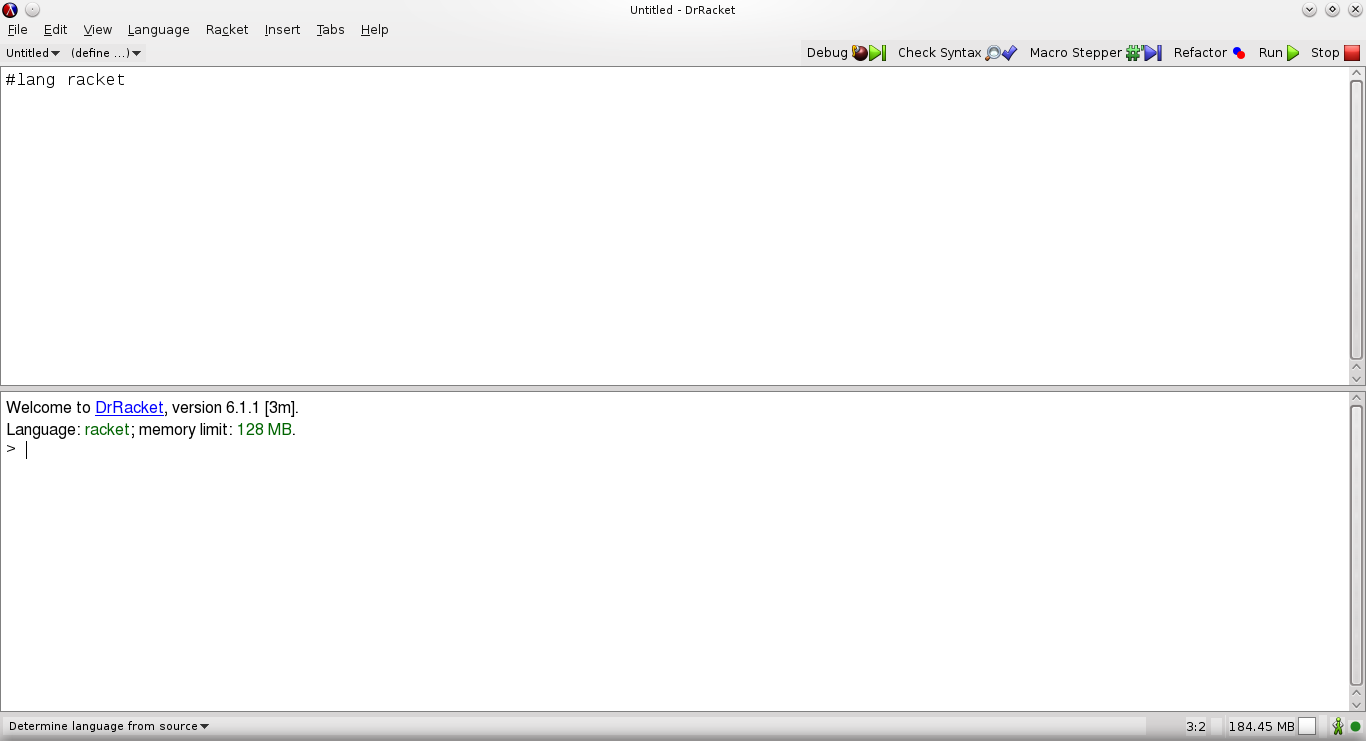
\includegraphics[width=0.95\textwidth]{img/DrRacketGui.png}
	\caption{DrRacket Graphical user interface}
	\label{fig:DrRacketGui}
\end{figure}

%Why Racket
%functional language, not many restructuring or refactoring are done for functional languages and less for racket
In order to do that we propose a implementation of a restructuring tool for Racket and Python for DrRacket where there are a lack of restructuring operations.


Racket \footnote{http://racket-lang.org/} programming language is a dialect of lisp and a descendant of Scheme and support objects, types and laziness evaluation,
whereas Python is a very high-level programming language that supports the imperative, functional and object-oriented programming paradigms and is very popular in many areas.


The restructuring will be implemented in the DrRacket, DrRacket is an integrated development environment (IDE), that was formerly known as DrScheme. It is a simple IDE that was initially build for Racket programming language and it is aimed at inexperienced programmers. ({\bf Fig.~\ref{fig:DrRacketGui}}).
It was designed as a pedagogic environment \cite{drscheme_pegadogy} and it was used in many introductory programming courses in schools around the world. In addition to that DrRacket supports development and extension of other programming languages \cite{tobin2011languages} and recently it have an implementation of python. \cite{ramos2014implementation}


The Section 2 addresses the objectives for this thesis work. Section 3 explore related work in refactoring and restructuring programs, some implemented restructuring tools and some implementations of language independent refactoring tools. Section 4 describes the architecture of the proposed solution. Section 5 explains how the tool will be evaluated and we conclude on section 6.



